\documentclass{article}
\usepackage{arxiv}

\usepackage[utf8]{inputenc}
\usepackage[english]{babel}
\usepackage[T1]{fontenc}
\usepackage{url}
\usepackage{booktabs}
\usepackage{amsfonts}
\usepackage{amssymb}
\usepackage{nicefrac}
\usepackage{hyperref}
\usepackage{microtype}
\usepackage{lipsum}
\usepackage{graphicx}
\usepackage{natbib}
\usepackage{doi}
\usepackage[colorinlistoftodos]{todonotes}
\usepackage{hyperref}

\renewcommand{\headeright}{Draft}
\renewcommand{\undertitle}{Draft}
\newcommand{\Hquad}{\hspace{0.5em}} 

\title{Detection of machine-generated fragments in text}

\author{ Anastasiya Voznyuk \\
	Department of Applied Informatics and Mathematics\\
	Moscow Institute of Physics and Technology\\
	\texttt{vozniuk.ae@phystech.edu} \\
	%\texttt{\href{https://colab.research.google.com/drive/1HBB8002s5_tFgFxGzIZQcBmsOsW6YcMh?usp=sharing} {Project code}} \\
    \\
    \textbf{Andrey Grabovoy} \\
	Moscow Institute of Physics and Technology\\
    Antiplagiat Company \\
	%% Address \\
	\texttt{grabovoy@ap-team.ru}}
	%% \And
	%% Coauthor \\
	%% Affiliation \\
	%% Address \\
	%% \texttt{email} \\
	%% \And
	%% Coauthor \\
	%% Affiliation \\
	%% Address \\
	%% \texttt{email} \\

\date{}

\renewcommand{\shorttitle}{Detection of machine-generated fragments in text}

%%% Add PDF metadata to help others organize their library
%%% Once the PDF is generated, you can check the metadata with
%%% $ pdfinfo template.pdf
\hypersetup{
pdftitle={A template for the arxiv style},
pdfsubject={q-bio.NC, q-bio.QM},
pdfauthor={Voznyuk Anastasiya},
pdfkeywords={Detection},
}

\begin{document}
\maketitle

\begin{abstract}
	This paper considers the problem of detecting machine-generated parts of text in the document. We introduce a model, that detects such text fragments and distinguishes their origin among several language models. To solve this problem we combine two models. The objective of the first one is to divide document into fragments of human-written text and machine-generated text. The second model aims to classify the generated fragments according to the language model from which they were obtained. In the computational experiment, we analyse the quality of such approach on dataset of documents with fragments generated by GPT-2, GPT, XLNet ans etc.
\end{abstract}


\keywords{Text Generation, Detection of Machine-generated text, Neural Authorship Attribution, Machine Learning, Natural Language Processing}

\section{Introduction}

% \cite{EVL:1}
In recent years there has been a rapid development of language models for text generation, transformers in particular, for example GPT~\cite{gpt}, GPT-2\cite{gpt2}, GPT-3~\cite{gpt3}, CTRL~\cite{ctrl} and mT5~\cite{mt5}. The problem of detecting machine-generated text has become more relevant recently due to the released ChatGPT\footnote{\url{https://openai.com/blog/chatgpt}} model by OpenAI. This model was trained on massive amounts of data and now is able to provide texts that are hardly distinguishable from human texts. The opposite task of detecting machine-generated text becomes more important due to many possible malicious usages of this technology. One can analyse the whole text or fragments of text.
We will focus on methods of subtracting the text-generated fragments in the set of documents.\\
With increased computational resources past statistical methods were applied to the novel detection problem. One of them was prediction entropy as an indicator of fake text, as described in~\cite{relativeentropy}. Also perplexity~\cite{perplexity} of the text, frequency of rare bigrams~\cite{rare_bigrams} or value of tf-idf~\cite{solaiman} can be taken into account. Another approach is to use classifiers that try to label given texts~\cite{Kuznetsov}.\\
For a long period recursive neural networks like LSTM were showing best results at solving the detection problem. In 2018 the mechanism of self-attention~\cite{Vaswani} was introduced and transformers have become new state-of-the-art approach.  Every new model has its own features and is usually trained on larger amounts of data, but attention mechanism always stays. These model can be used in detection of machine-generated text in two ways~\cite{solaiman}. The first method is using a language model that searches for artefacts from  methods, which most models are using for generating concise texts~\cite{gltr}. Additional training on new data is not required. The second method is based on fine-tuning on detection task. We fine-tune a language model to “detect itself”, using some stochastic methods, for example top-k, top-p sampling~\cite{gritsay2022}. 

Our approach consists of two steps. The first step is to divide each document into non-overlapping blocks of sentences. We take the baseline from work~\cite{Kuznetsov} on plagiarism detection.  We measure the quality of our model using metrics from text segmentation and plagiarism detection problems\cite{granularity}. We suppose, that within a fragment with artificial text there is a similar semantic structure.  The next step is to detect the origin of all the fragments, if they are machine-generated text. It can be done with transformer-based models, similar to \cite{gritsay2022}. This papers presents computational experiments with these models to combine them in one model and analyse the parameters on which the best performance will be obtained. Dataset will be constructed from existing datasets, such as GPT-2 output dataset\footnote{\url{https://github.com/openai/gpt-2-output-dataset}} and RUaTD competition dataset\footnote{\url{https://www.kaggle.com/competitions/ruatd-2022-multi-task/data}}.  %%%%---!!

\section{Problem statement}

Let $\mathbf{W}$ be our alphabet, tokens consists from characters from that alphabet.

Let $$\mathbb{D} = \Bigl\{\Big[t_j\Big]_{j=1}^n \Hquad|\Hquad t_j \in \mathbf{W}, n \in \mathbb{N}\Bigr\}$$ be the space of our documents.

We have a set of $N$ documents
$$\mathbf{D} = \bigcup_{i=1}^{N}D^i, D^i \in \mathbb{D}$$

%Each document  $D^i$ consists of $d_i$ tokens $t_1^i, t_2^i, ..., t_{d_i}^i$, where $t_j^i \in \mathbf{W}$ .
We have $K$ classes of our text-generative models, that generated fragments of text in $\mathbf{D}$.

We have $K + 1$ labels, that we use for multiclass classification, where $0$ is the label of human-written fragment, $\{1...K\}$ are the  labels that represent corresponding language model, let $\mathbf{C}$ be our set of labels.

Our model $\mathbf{\phi}$ is a superposition of two mappings, $\mathbf{f}$ and $\mathbf{g}$. Mapping $\mathbf{f}$ is responsible for text segmentation. Mapping $\mathbf{g}$ is responsible for classifying obtained fragments.

$$\mathbf{\phi} : \mathbf{g} \circ \mathbf{f},$$


$$\mathbf{\phi}: \mathbb{D} \rightarrow \mathbb{T}, \qquad \mathbb{T} = \Bigl\{\Big[t_{s_j}, t_{f_j}, C_j\Big]_{j = 1}^{J} \Hquad|\Hquad t_{s_j} = t_{f_{j - 1}},\Hquad s_j \in \mathbb{N}_0,\Hquad f_j \in \mathbb{N}, \Hquad C_j \in \mathbf{C}\Bigr\},$$

where $J$ is a number of fragments in segmentation of the document, $t_{s_j}$ is starting index of the $j$-th fragment,  $t_{f_j}$ is finishing index of the $j$-th fragment,  $C_{j}$ is class of the $j$-th fragment.



\subsection{Text fragmentation}
The first step is to divide our text into sequential non-overlapping fragments of different origin.

$$\mathbf{f}: \mathbb{D} \rightarrow \mathbf{T}^*, \qquad \mathbf{T}^* = \Bigl\{\Big[t_{s_j}, t_{f_j}\Big]_{j = 1}^{J}\quad|\quad t_{s_j} = t_{f_{j - 1}}, s_j \in \mathbb{N}_0, f_j \in \mathbb{N}\Bigr\},$$

where $s_j$ is start of the $j$-th fragment and $f_j$ is end of the $j$-th fragment.

Thus, $\mathbf{T}^*$ is a set of all possible sequences of non-overlapping blocks of texts, that covers complete document.

We assume that in each document the blocks of text with the same origin are big enough. Thus, we search for style changes on sentence level. Style change indicates that several next sentences starting from the beginning of the style change have different origin. Each sentence receives  label $\textbf{0}$ or $\textbf{1}$, where $\textbf{0}$ means it is a human-written sentence and $\textbf{1}$ is a machine-generated sentence in case of binary classification, and corresponding $K$ labels in case of multiclass classification. A fragment is a sequence of neighbouring sentences of maximum possible length, that have the same label. We repeat this process for every document in given set of documents. 
 
We extract features from sentences in the document and get feature vectors. Our goal is to cluster groups of fragments of the same author, thus we need to maximise the clusterability of the feature vectors.
Let $(\vect{v}_i)_{i=1}^n$ be a sequence of basic feature vectors with elements from $\mathbb{R}^{n_{v}}$. We apply a transformation to these vectors to ease the process of following clustering of these vectors.
$$T:\mathbb{R}^{n_\mathrm{v}}\rightarrow\mathbb{R}^{n_\mathrm{t}},$$
$$T(\vect{x}) &= \textbf{\matr{W}}\vect{x},$$
where $\textbf{\matr{W}}\in \mathbb{R}^{n_\mathrm{v}\times n_\mathrm{t}}$. 
Let $(l_i)_{i=1}^n$ be the sequence of true author labels with elements from $\textbf{C}$. 

To optimise the transformation $T$, we use the center loss function\cite{clf}:
\begin{equation}
	L_\mathrm{c} &= \sum_{c = 0}^{K + 1}\frac{1}{N_c} 
		\sum_{i=1}^{n} \| T(\vect{v}_i)-\vect{\mu}_{c}\|^2 [l_i=c],
\end{equation}

where $N_c = \sum_{i=1}^n[l_i=c]$ is the number of sentences labeled with author $a$ and $\vect{\mu}_c$ represent the current centroid of the transformed feature vectors associated with the author label $c \in \textbf{C}$:
\begin{equation}
\vect{\mu}_c = \frac{1}{N_c}\sum_{i=1}^n T(\vect{v}_i)[l_i=c].
\end{equation}	


\subsection{Fragment classification}

The second step is to classify each fragment with label from $\mathbf{C}$
$$\mathbf{g}: \mathbf{T}^* \rightarrow \mathbf{C}.$$

We apply that function to every text fragment, obtained from the previous step. This is a classical multi-classification task. We will use cross-entropy as a loss function:

$$Loss_{cls}(x) = \sum_{i=0}^K-p(x)\log q(x)$$ 
where $p(x)$ is probability of object $x$ to be actually labelled with $i$,
$q(x)$ is  probability of object $x$ to be labelled with $i$  in prediction.

\subsection{Performance criteria}

To measure how good our model is capable to divide our documents into fragments we will use metric, used in PAN Competition\cite{granularity} measurements.
Let $S$ be our true segmentation and $\hat{S}$  is the predicted segmentation. We divide the segments from the true segmentation $S$ and the predicted segmentation $\hat{S}$ each into sets of segments $S_i$, $i\in\{1..c\}$, and $\hat{S}_j$, $j\in\{1..\hat{c}\}$, where $c$ is the true number of authors, and $\hat{c}$ the predicted number of authors.  Precision of an item is the proportion of items in its cluster which have the item’s label, including itself. In our tasks item is a segment from a document, extracted by model.  
$$ prec(S, R) = \frac{1}{|R|}\sum_{r \in R}\frac{|\bigcup_{s \in S}(s \cap r)|}{|r|},$$

$$ rec(S, R) = \frac{1}{|S|}\sum_{s \in S}\frac{|\bigcup_{r \in R}(s \cap r)|}{|s|},$$


Another metric is granularity, which measures whether our model detects a segment of different origin as a whole or in several segments.

$$ gran(S, R) = \frac{1}{|S_{R}|}\sum_{s \in S_{R}}|R_{S}|,$$

where $S_{R} \subseteq S$ denotes proved change of author in $R$, and $R_{S} \subseteq R$ are alleged changes of author in $s$.

\section{Computational Experiment}


Our task of text segmentation of subdivided by 2 task. The first one is binary classification and the second one is multiclass classification.


The goal of computational experiment is to analyse how good our solution is at segmenting fragments of text and classifying them. 

% RuATD competition, which provided the dataset, also provided accuracy score for their baseline solutions. One solution uses tf-idf + logistic regression approach, the other solution uses fine-tuned BERT. We will use a modification of the second approach and compare our results with the ones, suggested by the authors of competition.
% The task is to find the optimal parameters of our model in which certain requirements on the quality of the model will be achieved.
% For text fragmentation we use Gradient Boosting Regression Tree for classifying the sentences, as described in \cite{Kuznetsov}. The optimal parameters are (???).
% %(n_estimators=200, max_depth=4)%
% %by maximization of the Area-Under-Curve classification measure.
% Also we detect outliers: if a sentence is label-classified with some value higher than threshold, we will label it as a machine generated sentence.

% For fragment classification we suggest to use an approach, described in \cite{gritsay2022}, namely RoBERTa-base model for English texts and XLM-RoBERTa-base model for Russian texts.

\subsection{Dataset}

For binary segmentation we generate a dataset of 10000 documents, each of documents consists of 5-6 fragments of different origin, either human-authored or machine-authored. Human-written fragments were taken from Wikipedia Dataset \footnote{\url{https://huggingface.co/datasets/wikipedia}}.Machine-generated texts were generated by GPT-2 model\footnote{\url{https://github.com/openai/gpt-2-output-dataset}}.

For multiclass segmentation we separately generated datasets of 2000 documents with fixed number of language models, participating in creating those fragments. This number varies from 3 to 5. Machine-generated texts for multiclass classification problem were generated by 8 models as described in \cite{uchendu-etal-2020-authorship}. Statistics for each model and percent of its presence in texts is described in Appendix 1. \\

% We conducted further classification only for binary segmentation as multiclass segmentation already labels the fragments with suggested authors. 

Further classification is done on the same datasets, that were created for multiclass segmentation, but processed with binary segmentation pipeline.


% For our experiment with classification we took the data, that was collected for RUATD 2022 competition\cite{ruatd-dataset} for multitask classification. The test dataset contains 215105 short fragments, that were generated by different 13 models. Authors claim that various language models fine-tuned on different tasks: machine translation, paraphrasing, summarization, simplification and unconditional text generation - were used to generate texts. Moreover, the part of the set was annotated automatically by different generative models. Among models there are several versions of ruGPT, mT5 and ruT5 and M-BART.

\subsection{Configuration of algorithm of segmenting}

Pipeline for extracting segments from the document consists of tokenization of sentences, basic feature extraction, feature transformation and clustering. 

Parameters are randomly initialized with values from a truncated normal distribution with standard deviation $0.1$. It is trained using RMSProp optimizer with learning rate $10^{-5}$.

Feature extraction was conducted with a sliding window that includes context of each token. The size of sliding window is 120 tokens. Among features, that were extracted, were stop word counts, Bag of Words, character trigram counts. After that we transformed these features with a linear layer. We trained weight matrix for transformation, using RMSProp as optimizer with learning rate $10^{-5}$. Clustering was done with AutoKMeans algorithm from \texttt{sklearn} library.

\subsection{Configuration of algorithm of classifaction}
For tokenization of sentences in text fragments we used pretrained embedding from \texttt{bert-base-multilingual-cased}\footnote{\url{https://github.com/google-research/bert/blob/master/multilingual.md}}. The same model was fine-tuned for our sequence classification task. We trained our model for 3 epochs. For optimization we used AdamW optimization algorithm\cite{adam-w}.


% The dataset, PAN-PC-11\cite{pan-dataset} was intended to use for intrinsic plagiarism detection. We will analyse our task on sentence-level, this will be out tokens. The test collection consists of 4753 documents and is split into 10 folds. Each folds contains 500 documents except for the smaller fold 10. We used it as a benchmark for measuring, how good our model is in fragmenting a document.

% The dataset, used for text classification problem was GPT-2 output dataset\cite{gpt2-dataset}, which allows  to compare data from models with different numbers of parameters and different sampling methods. 

% For evaluating our task we will need to generate our own dataset with document by taking fragments from this dataset and from RUaTD task dataset \cite{ruatd-dataset} and combining them with fragments of human-written text. However, one should be careful when generating a document, we need to pay attention and do not let our generator to take fragments from different domains. 


  
\section{Conclusion}

On binary segmentation on 3000 documents we receive following metrics: precision equals 0.8017, recall is 0.4247, granularity is equal 1.4386. Our model is rather good at distinguising human fragments from machine-generated ones, but has a poor quality on finding machine-generating fragments. Granularity is close to 1, which shows, that model is not tend to detect one large segment by smaller parts of it, but rather detects it as a whole fragment. 

For problem of multiclass segmentation various metrics, such as precision, recall and granularity can be viewed on Figure 3, Figure 4 and Figure 5.  On the contrary, for all possible number of authors our model showed low precision, but high recall. We received the largest recall on 5 authors equal to 0.94, then recall drops to 0.89 for 4 authors and drops again to 0.86 for 3 authors. Granularity equals to 7.5 is extremely high for dataset with 5 authors, which means it tends to extract very small segments, For 4 and 3 authors it does not change very much between each other, but 4.5 is still a large value for given metric.

We received 56$\%$ of accuracy with 3 epoch of training only using the part of the dataset. It is less than the score, provided by the authors of competition, which is 59$\%$, but this difference is explained by smaller size of the dataset. Also we may suggest that due to increasing loss on validation set, our model started to overfit. Another issue with the quality of classification on some classes: for some classes there's a small recall, e.g class 6. For some classes there's both small recall and small precision, e.g class 3, class 12 and class 13. For some of class it is happened because of small amount of these classes in dataset. 

\section{Discussion}

Our model performs well at task of binary classification, but there are some problems, that need to be figured out and resolved.


\begin{table}[bhtp]
	\centering
	\caption{Table of train accuracy and validation accuracy on each epoch}
	\label{tbl:space_and_subspace}
	\begin{tabular}{| c | c | c | c | }
		\hline
		Number of epoch & Train. loss & Valid.loss & Valid. accuracy \\
		\hline
		1 & 1.30  & 1.26 & 0.54  \\
        \hline
		2 & 1.07 & 1.27 & 0.56  \\
		\hline
        3 & 0.86  & 1.35 & 0.56  \\
        \hline
	\end{tabular}
\end{table}

\begin{figure}[bhtp]
	\includegraphics[width=\textwidth]{Unknown-2.png}
	\caption{Graph of validation / train loss versus epoch}
	\label{fig:1}
\end{figure}


\begin{figure}[bhtp]
	\includegraphics[width=\textwidth]{Unknown.png}
	\caption{Graph of Precision-Recall Curve for every class}
	\label{fig:2}
\end{figure}

\begin{figure}[bhtp]
	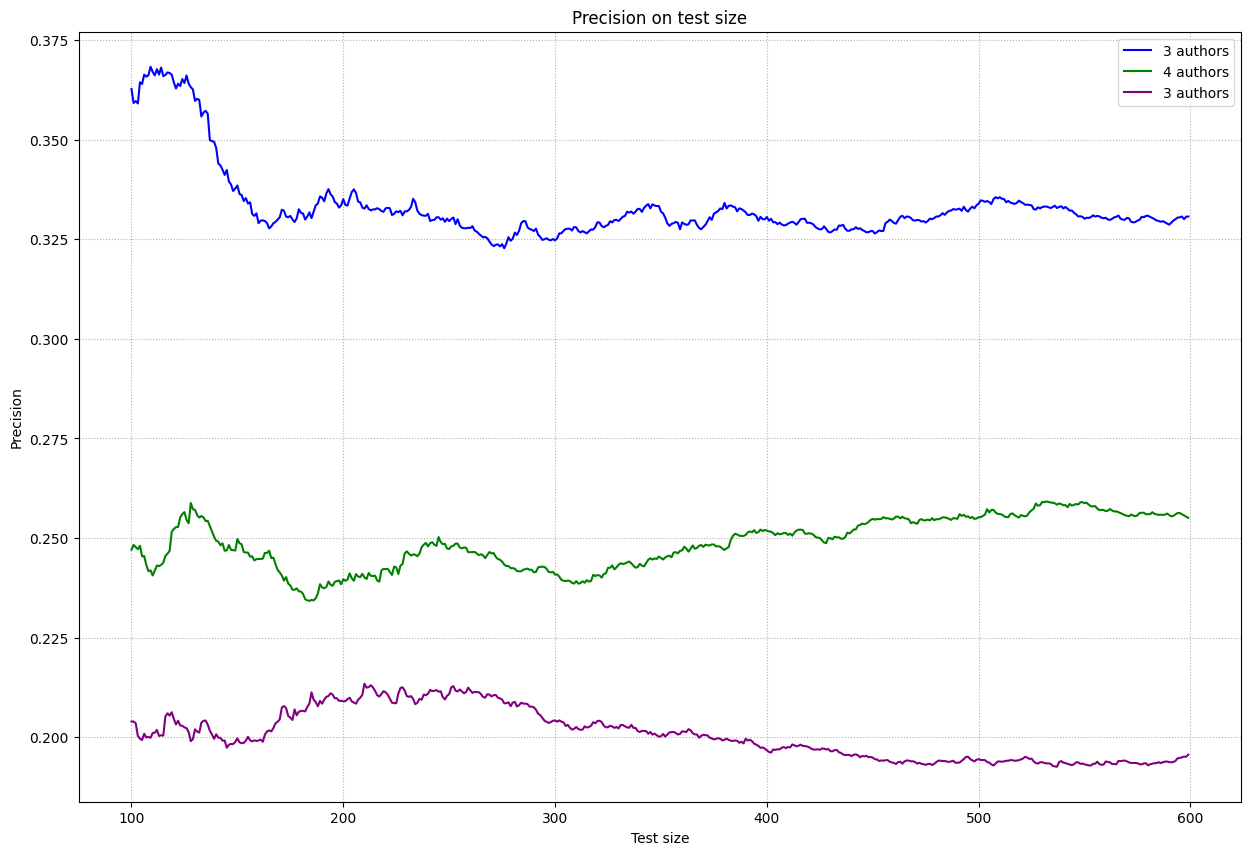
\includegraphics[width=\textwidth]{pr.png}
	\caption{Graph of Precision of Multiclass Fragmenting}
	\label{fig:3}
\end{figure}

\begin{figure}[bhtp]
	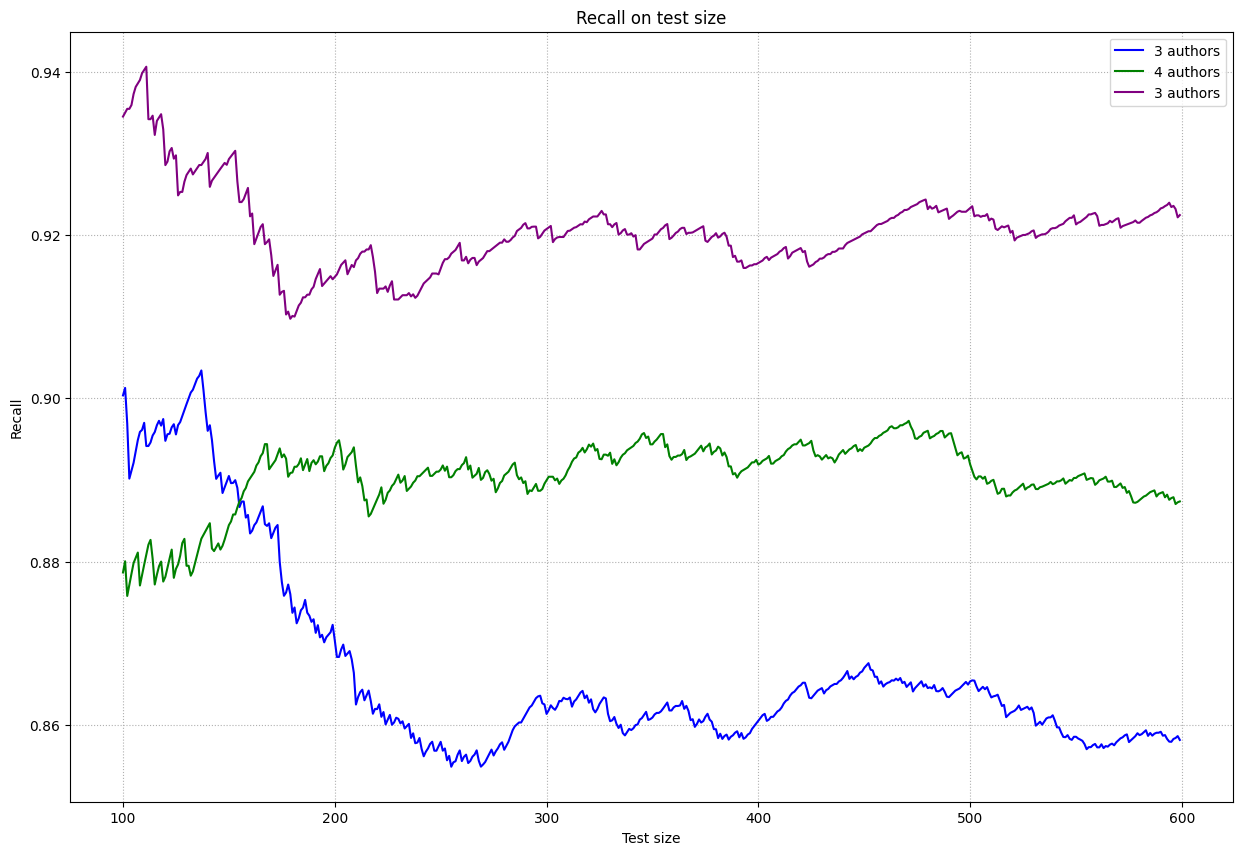
\includegraphics[width=\textwidth]{rc.png}
	\caption{Graph of Recall of Multiclass Fragmenting}
	\label{fig:4}
\end{figure}

\begin{figure}[bhtp]
	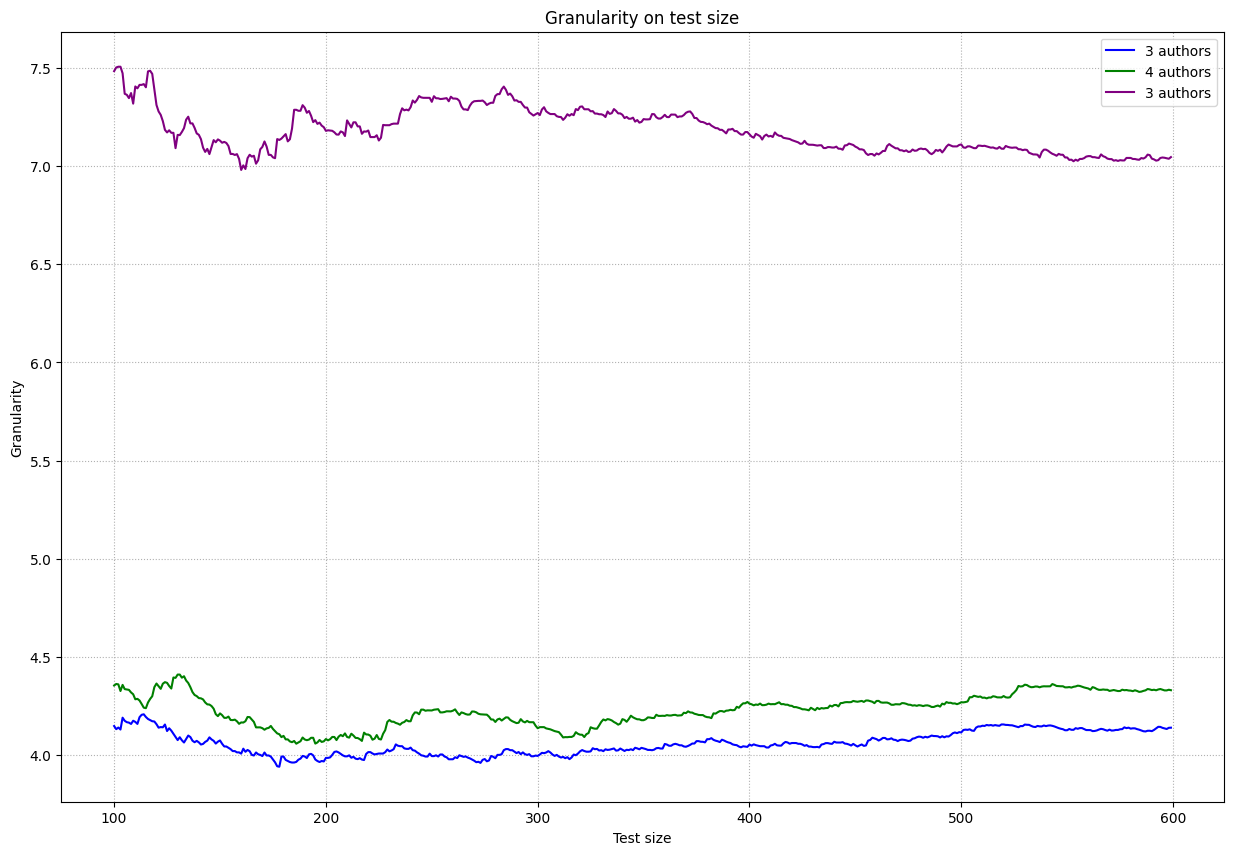
\includegraphics[width=\textwidth]{gr}
	\caption{Graph of Granularity of Multiclass Fragmenting}
	\label{fig:5}
\end{figure}



% \begin{figure}[bhtp]
% 	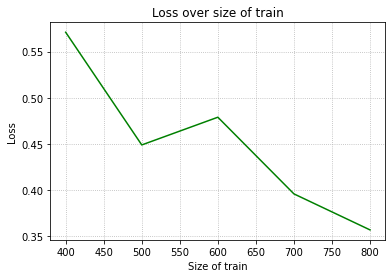
\includegraphics[width=\textwidth]{loss.png}
% 	\caption{Graph on Loss Function}
% 	\label{fig:3}
% \end{figure}

\clearpage
\bibliographystyle{plain}
\bibliography{references}

\newpage
\appendix
\section{Multiclass Segmentation}

In the task of segmenting text with fragments generated by several language models we used 8 models: XLNet~\cite{xlnet}, GPT-2~\cite{gpt2}, PPLM~\cite{pplm}, GPT~\cite{gpt}, GROVER~\cite{grover}, FAIR~\cite{FAIR}, XLM~\cite{xlm}, CTRL~\cite{ctrl}.

We generate  documents with 3, 4, 5 different authors, as we want each document to contain only 5-6 fragments. For every number of authors we create 2000 documents and for each document we sampled 3 participants and then 6 times sample author of next fragment. If on some step we sample the same author from previous step, we resample it until received different author. 

\begin{figure}[bhtp]
	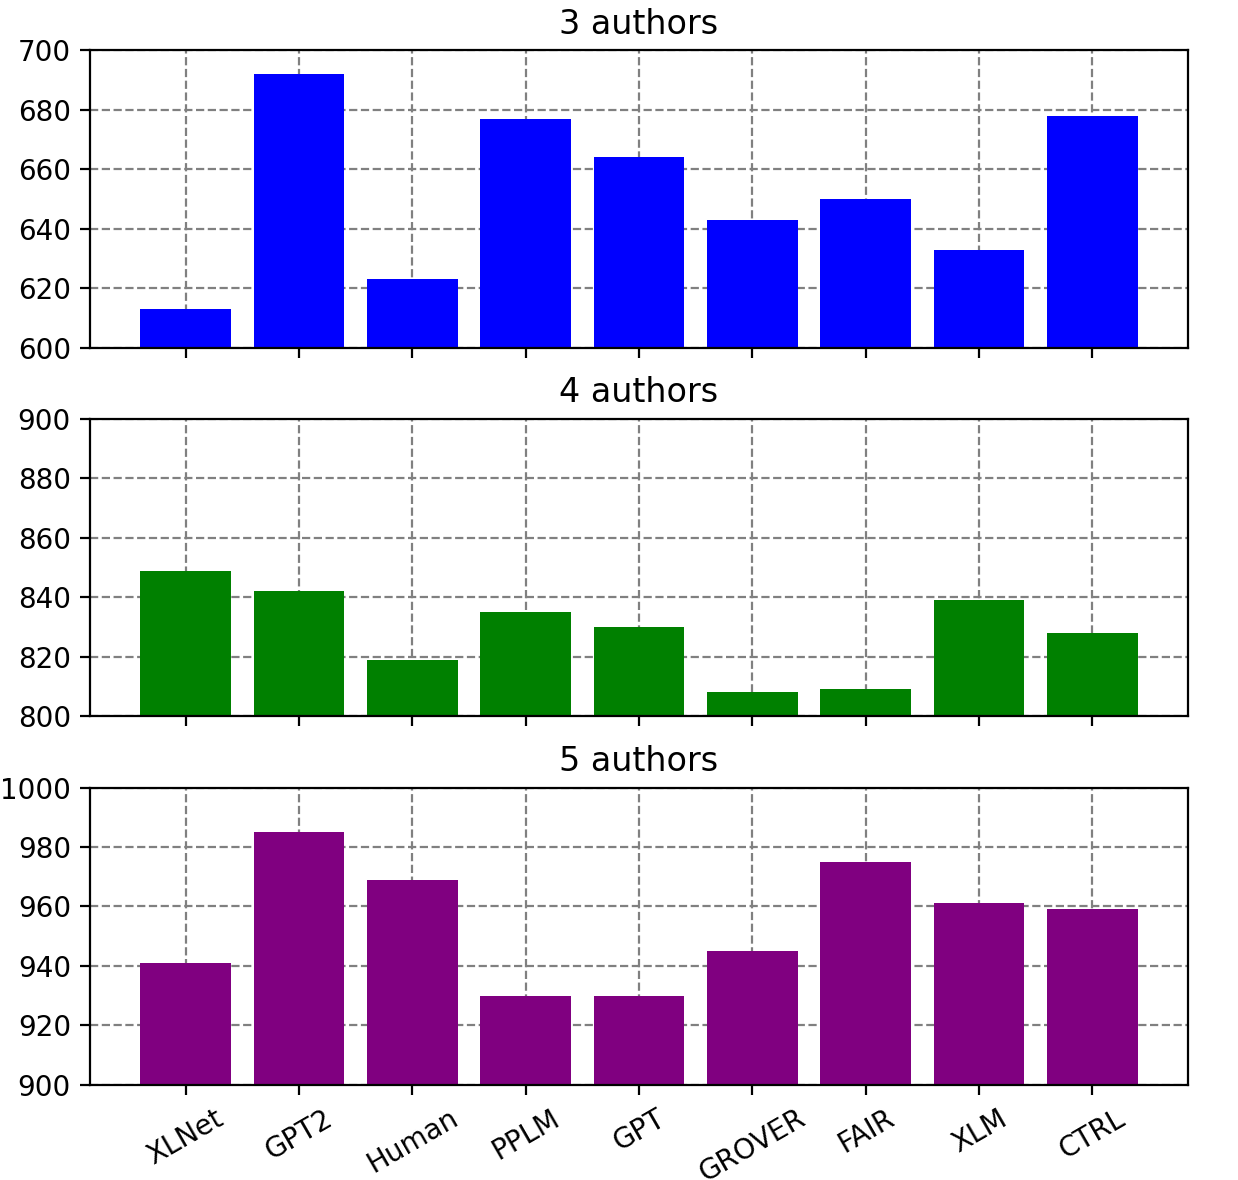
\includegraphics[width=\textwidth]{authors_1.png}
	\caption{Statistics on language models as authors occurrence in generated files}
	\label{fig:6}
\end{figure}

We can see the least differences among authors' occurrences is for 4 authors, while the largest is for 3 authors.

\section{List of figures and tables}
\begin{enumerate}
    \item Table of train accuracy and validation accuracy on each epoch
    \item Validation / train loss versus epoch - Figure 1
    \item Precision-Recall Curve for every class - Figure 2
    \item Precision of Multiclass Fragmenting - Figure 3
    \item Recall of Multiclass Fragmenting - Figure 4
    \item Granularity of Multiclass Fragmenting - Figure 5
    \item Statistics on language models as authors occurrence in generated files - Figure 6
    
\end{enumerate}
\end{document}